% ======================================================================
\section{Electrostatics of the stack: the layer-resolved Coulomb kernel}
\label{sec:electrostatics}
% ======================================================================

\subsection{Geometry}

$N$ sheets $\ell=0,\dots,N-1$ sit at heights $z_0>z_1>\dots>z_{N-1}$ and divide space into $N+1$ regions
(\cref{fig:stack}): region $0$ above sheet $0$, region $j$ ($1\le j\le N-1$) between sheets $j-1$ and $j$,
of thickness $d_{j-1}=z_{j-1}-z_j$ (\code{d[j-1]} in the code), and region $N$ below sheet $N-1$. The outer
regions are half-spaces, or are terminated by grounded gates at distances $d_{\rm t}$ above sheet $0$ and
$d_{\rm b}$ below sheet $N-1$ (\code{top\_gate\_d}, \code{bottom\_gate\_d}), or (top only) by a slab of
thickness $d_{\rm s}$ backed by a half-space $\varepsilon_{\rm c}$ (\code{CappedLayerCoulomb}).

\begin{figure}[h]
\centering
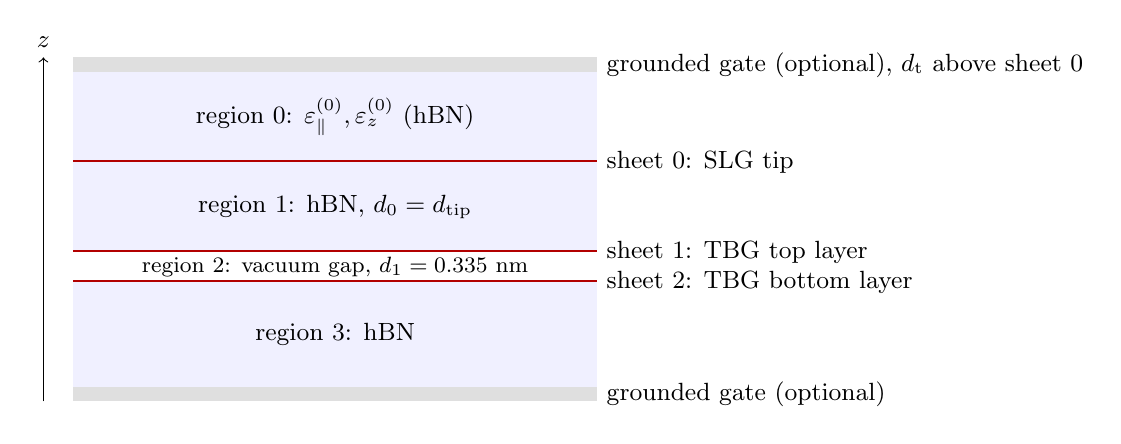
\begin{tikzpicture}[scale=0.95, every node/.style={font=\small}]
\fill[gray!25] (0,4.4) rectangle (7,4.6); \node[right] at (7,4.5) {grounded gate (optional), $d_{\rm t}$ above sheet 0};
\fill[blue!6] (0,3.2) rectangle (7,4.4); \node at (3.5,3.8) {region 0: $\varepsilon^{(0)}_\parallel,\varepsilon^{(0)}_z$ (hBN)};
\draw[very thick, red!70!black] (0,3.2) -- (7,3.2); \node[right] at (7,3.2) {sheet 0: SLG tip};
\fill[blue!6] (0,2.0) rectangle (7,3.2); \node at (3.5,2.6) {region 1: hBN, $d_0=d_{\rm tip}$};
\draw[very thick, red!70!black] (0,2.0) -- (7,2.0); \node[right] at (7,2.0) {sheet 1: TBG top layer};
\fill[white] (0,1.6) rectangle (7,2.0); \node at (3.5,1.8) {\footnotesize region 2: vacuum gap, $d_1=0.335$ nm};
\draw[very thick, red!70!black] (0,1.6) -- (7,1.6); \node[right] at (7,1.6) {sheet 2: TBG bottom layer};
\fill[blue!6] (0,0.2) rectangle (7,1.6); \node at (3.5,0.9) {region 3: hBN};
\fill[gray!25] (0,0.0) rectangle (7,0.2); \node[right] at (7,0.1) {grounded gate (optional)};
\draw[->] (-0.4,0) -- (-0.4,4.6) node[above] {$z$};
\end{tikzpicture}
\caption{The three-sheet stack used for the TBG sample (notebooks 03, 05). For SLG$|$hBN$|$SLG there are two
sheets and three hBN regions.}
\label{fig:stack}
\end{figure}

\subsection{Poisson equation in one region}

With $\bm E=-\nabla\phi$, $\bm D=\bm\varepsilon\bm E$ and $\nabla\cdot\bm D=4\pi\rho$, a 2D Fourier transform
in the plane gives, inside region $j$ (no free charge),
\begin{equation}
\varepsilon_z^{(j)}\partial_z^2\phi-\varepsilon_\parallel^{(j)}q^2\phi=0
\quad\Rightarrow\quad
\phi''=\kappa_j^2\phi,\qquad
\kappa_j=q\sqrt{\varepsilon_\parallel^{(j)}/\varepsilon_z^{(j)}},\qquad
Y_j=\varepsilon_z^{(j)}\kappa_j=q\sqrt{\varepsilon_\parallel^{(j)}\varepsilon_z^{(j)}} .
\label{eq:kappaY}
\end{equation}
$Y_j$ is the \emph{admittance} of the region (\code{compute\_kappa\_Y}). For a spacer of thickness $d$
whose lower and upper faces are at potentials $\Phi_b$ and $\Phi_a$, the solution
$\phi(z)=[\Phi_a\sinh\kappa z+\Phi_b\sinh\kappa(d-z)]/\sinh\kappa d$ ($0\le z\le d$) gives the normal
displacement on the two faces:
\begin{equation}
\varepsilon_z\phi'(d^-)=Y\bigl[\Phi_a\coth\kappa d-\Phi_b\csch\kappa d\bigr],\qquad
\varepsilon_z\phi'(0^+)=Y\bigl[\Phi_a\csch\kappa d-\Phi_b\coth\kappa d\bigr].
\label{eq:spacer}
\end{equation}
For a half-space above sheet $0$, $\phi=\Phi_0e^{-\kappa(z-z_0)}$ and $\varepsilon_z\phi'=-Y_0\Phi_0$; with a
grounded gate at distance $d_{\rm t}$, $\phi=\Phi_0\sinh\kappa(z_{\rm g}-z)/\sinh\kappa d_{\rm t}$ and
$\varepsilon_z\phi'=-Y_0\coth(\kappa d_{\rm t})\,\Phi_0$. A gate therefore replaces the boundary admittance
$Y\to Y\coth(\kappa d_{\rm g})$, which tends to $Y$ for $d_{\rm g}\to\infty$. A slab
$(\kappa_s,Y_s,d_s)$ capped by a half-space with $Y_c=\varepsilon_cq$ gives instead
\begin{equation}
Y_{\rm eff}=Y_s\,\frac{Y_c+Y_s\tanh\kappa_sd_s}{Y_s+Y_c\tanh\kappa_sd_s},
\label{eq:capped}
\end{equation}
which interpolates between $Y_c$ ($d_s\to0$), $Y_s$ ($d_s\to\infty$) and the gate result ($Y_c\to\infty$)
(\code{capped\_slab\_admittance}).

\subsection{Matching at the sheets: the tridiagonal admittance matrix}

The potential is continuous across sheet $\ell$ and the displacement jumps by the sheet charge,
$D_z(z_\ell^+)-D_z(z_\ell^-)=4\pi\sigma_\ell$, i.e.\
$-\varepsilon_z\phi'(z_\ell^+)+\varepsilon_z\phi'(z_\ell^-)=4\pi\sigma_\ell$. Inserting \cref{eq:spacer} for
the regions above (region $\ell$) and below (region $\ell+1$) sheet $\ell$:
\begin{equation}
\bigl[Y_\ell\coth\kappa_\ell d_{\ell-1}+Y_{\ell+1}\coth\kappa_{\ell+1}d_\ell\bigr]\Phi_\ell
-Y_\ell\csch(\kappa_\ell d_{\ell-1})\,\Phi_{\ell-1}
-Y_{\ell+1}\csch(\kappa_{\ell+1}d_\ell)\,\Phi_{\ell+1}=4\pi\sigma_\ell ,
\end{equation}
with the outermost terms replaced by the boundary admittances ($Y_0$, $Y_0\coth\kappa_0d_{\rm t}$ or
$Y_{\rm eff}$ on top; $Y_N$ or $Y_N\coth\kappa_Nd_{\rm b}$ at the bottom). This is
$A(q,\omega)\Phi=4\pi\sigma$ with a tridiagonal $A$ (\code{build\_tridiagonal\_A\_diagonals}):
\begin{align}
A_{00}&=Y_{\rm top}+Y_1\coth\kappa_1d_0, &
A_{N-1,N-1}&=Y_{N-1}\coth\kappa_{N-1}d_{N-2}+Y_{\rm bot},\nonumber\\
A_{\ell\ell}&=Y_\ell\coth\kappa_\ell d_{\ell-1}+Y_{\ell+1}\coth\kappa_{\ell+1}d_\ell, &&\nonumber\\
A_{\ell,\ell-1}&=-Y_\ell\csch\kappa_\ell d_{\ell-1}, &
A_{\ell,\ell+1}&=-Y_{\ell+1}\csch\kappa_{\ell+1}d_\ell .
\label{eq:Amatrix}
\end{align}
A unit point charge $e$ on sheet $m$ has $\sigma_\ell(\bq)=e\,\delta_{\ell m}$, and the energy of a second
charge $e$ on sheet $\ell$ is $e\Phi_\ell$. The layer-resolved Coulomb kernel is therefore
\begin{equation}
\boxed{V_{\ell m}(q,\omega)=4\pi e^2\,[A^{-1}(q,\omega)]_{\ell m}}
\qquad[\text{eV\,nm}^2]
\label{eq:V}
\end{equation}
(\code{LayerCoulomb.coulomb\_matrix}). $A$ is inverted with a Thomas LU factorisation and $\coth$, $\csch$
are evaluated in the overflow-safe form $\coth z=(1+u)/(1-u)$, $\csch z=2e^{-z}/(1-u)$, $u=e^{-2z}$, with
$1-u=-\mathrm{expm1}(-2z)$.

\paragraph{Closed forms (tested).} A single sheet in a uniform medium has $A=2\varepsilon q$, i.e.\
$V=2\pi e^2/(\varepsilon q)$; with gates at $\pm d$, $V=\frac{2\pi e^2}{\varepsilon q}\tanh qd$; with one gate,
$V=\frac{2\pi e^2}{\varepsilon q}(1-e^{-2qd})$. Two sheets in a uniform uniaxial medium:
\begin{equation}
V_{11}=V_{22}=\frac{2\pi e^2}{\bar\varepsilon q},\qquad V_{12}=V_{11}\,e^{-\kappa d},
\qquad \bar\varepsilon=\sqrt{\varepsilon_\parallel\varepsilon_z},\quad\kappa=q\sqrt{\varepsilon_\parallel/\varepsilon_z}.
\label{eq:bilayerV}
\end{equation}

\subsection{Bilayer channels and the effect of gates}
\label{sec:channelsV}

For two equivalent sheets, $V$ is diagonalised by $u_\pm=(1,\pm1)/\sqrt2$ with eigenvalues
$V_\pm=V_{11}\pm V_{12}$. At $qd\ll1$, $V_+\simeq 4\pi e^2/(\bar\varepsilon q)$ (the total charge sees the
long-range Coulomb field) while $V_-\simeq V_{11}\kappa d=2\pi e^2 d/\varepsilon_z$ is finite (a dipole layer).
$V_+$ drives the in-phase (optical, $\omega\propto\sqrt q$) plasmon and $V_-$ the out-of-phase (acoustic,
$\omega\propto q$) plasmon. Gates at distance $d_{\rm g}$ cut the long-range part,
$V_+\to 4\pi e^2 d_{\rm g}/\varepsilon_z$ for $qd_{\rm g}\ll1$ (gates at $\pm d_{\rm g}$), but leave $V_-$ almost unchanged when
$d\ll d_{\rm g}$: gating raises the \emph{relative} weight of the acoustic channel by suppressing the optical one
(notebook 01, test \code{test\_gate\_suppresses\_in\_phase\_more\_than\_out\_of\_phase}).

\subsection{Dispersive dielectrics and passivity}

hBN is modelled with one Lorentz oscillator per axis,
\begin{equation}
\varepsilon_\alpha(\omega)=\varepsilon_{\infty,\alpha}+\frac{\varepsilon_{0,\alpha}-\varepsilon_{\infty,\alpha}}{1-\omega^2/\omega_{T,\alpha}^2-\ii\gamma_\alpha\omega/\omega_{T,\alpha}^2},
\end{equation}
with $(\varepsilon_0,\varepsilon_\infty,\omega_T,\gamma)=(6.41,4.53,168,0.82)$ (in-plane) and
$(3.0,2.5,94.2,0.23)$ (out-of-plane), energies in meV (\code{dielectrics.HBNModel}). Between $\omega_T$ and
$\omega_L=\omega_T\sqrt{\varepsilon_0/\varepsilon_\infty}$ (the Reststrahlen bands, 94--103 meV and
168--200 meV) $\varepsilon_\parallel\varepsilon_z<0$ and $\kappa$ is almost imaginary: the substrate carries
hyperbolic phonon polaritons and $V$ acquires a large dissipative part. For the retarded kernel of a passive
medium the anti-Hermitian part must be negative semidefinite, $-(V-V^\dagger)/2\ii\succeq0$. The branch of
$\kappa_j(\omega)$ is the decaying one ($\Ree\kappa>0$) at the first frequency of a sweep and is then
continued without jumps (\code{compute\_kappa\_Y\_tracked}); in the examples of notebook 01 the continued
and the principal branches coincide and both are passive. Static values ($\omega\to0$) are used unless the
phonon range is of interest (all calculations in notebooks 02--05).
